% !TeX root = Body.tex

\chapter{Velocity-driven Non-equilibrium Phase Transition in Ising Models}\label{ch:review}

Two moving magnets sometimes gain their magnetic orders at a higher temperature than its equilibrium case. Using an exactly solvable model,Hucht \cite{Hucht2009b} showed the existence of non-equilibrium phase transitions in Ising spin systems, which strongly depended on their spatial dimensionality. It is necessary to understand these non-equilibrium phase transitions for each spatial dimension because manipulating the magnetic friction strongly depends on its spatial dimensionality. We will find a dimensional crossover of the friction in Chap.~\ref{chap:Res}.

In this chapter we make a brief review of the exact results by Hucht \cite{Hucht2009b}. His analysis is based on the fact that two Ising cylinders with relative motion make a novel mean-field, which leads the system to a non-trivial phase transition.

\section{Overview of the results}

Let us consider two equivalent square lattices of the Ising model each of which contacts the other by one of its one-dimensional boundaries (see Fig.~\ref{fig:SketchNEIsing}). We make one lattice slide along the contact plane against the other lattice with a constant velocity $v$. The entire system thereby goes into a non-equilibrium stationary state instead of equilibrium. The stationary state well describes the behavior of two magnetic materials with a friction. We use this setup in Chapter~\ref{chap:NumSim}.

\begin{figure}[htbp]
	\centering
	\subcaptionbox{\label{subcap:one-dim}}[0.49\linewidth]{\raisebox{.70\height}{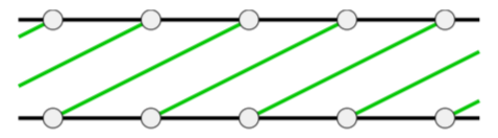
\includegraphics[width=0.35\linewidth]{Fig2Modified.pdf}}}
	\subcaptionbox{\label{subcap:two-dim}}[0.49\linewidth]{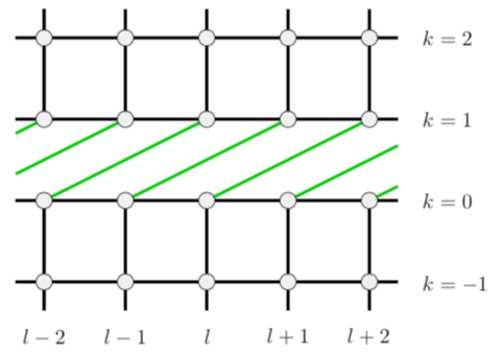
\includegraphics[width=0.35\linewidth]{Fig3Modified.pdf}}
	\caption{Sketches of the models considered in Ref.~\cite{Hucht2009b}\protect\footnotemark. Both cases depict a schematic view after the sliding by twice a lattice constant: (\subref{subcap:one-dim}) Two chains of the one-dimensional model; (\subref{subcap:two-dim}) Two square lattices of the two-dimensional model. Letters $k$ and $l$ denote the coordinates on $z$ and $x$ axises, respectively.}
	\label{fig:SketchNEIsing}
\end{figure}

\footnotetext{Reprinted Figs.~2 and 3 with permission from \fullcite{Hucht2009b}. Copyright (2018) by the American Physical Society.}

As a well known fact, the ordinary two-dimensional Ising model has an equilibrium phase transition at the critical temperature $T_{\rm c,eq}=2/\left[\log\left(1+\sqrt{2}\right)\right]=2.2691853\dots$ in the thermodynamical limit. The system with the friction reduces to the equilibrium case in the limit of $v\to 0$. For finite velocity, it was revealed \cite{Kadau2008,Hucht2009b} that there exists above the equilibrium critical point a novel phase transition in which the magnetization grows on the sliding boundary (see Fig.~\ref{fig:NEPTinIsing}). Let us denote the velocity-dependent non-equilibrium critical point by $T_{\rm c}(v)$ apart from the equilibrium critical point $T_{\rm c, eq}$. Hucht \cite{Hucht2009b} claimed that the critical temperature $T_{\rm c}(v)$ \textit{deviates} from $T_{\rm c,eq}$ at the point $v=0$ towards the limit $v=\infty$.

\begin{figure}[htbp]
\centering
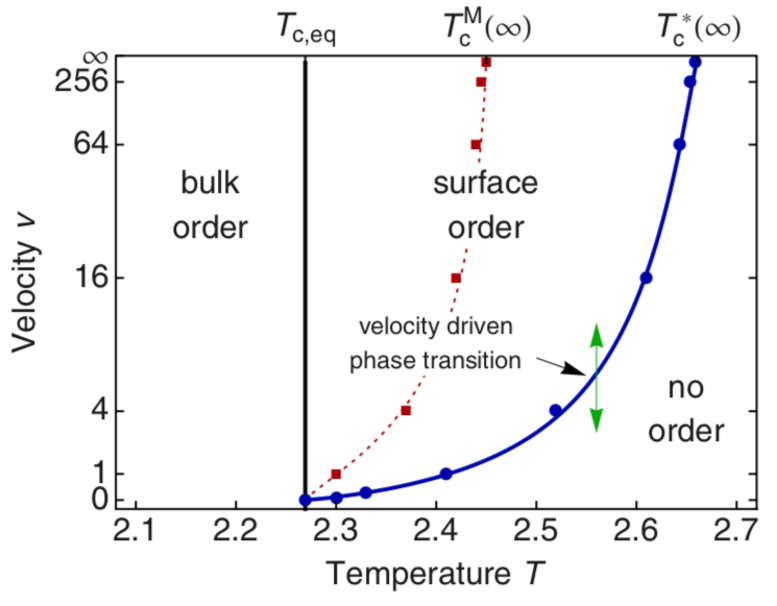
\includegraphics[width=0.5\linewidth]{Fig15.pdf}
\caption{The phase diagram of the two-dimensional non-equilibrium Ising model obtained in Ref.~\cite{Hucht2009b}\protect\footnotemark. The black solid line, the red dashed line and the blue solid line indicate the ordinary bulk phase transition $T_{\rm c,eq}$, a non-equilibrium boundary phase transition for the Metropolis rate $T_{\rm c}^{\rm M}(v)$ and one for the multiplicative rate $T_{\rm c}^{*}(v)$, respectively. Crossing from the right to the left across the non-equilibrium phase boundary, the system acquires a non-zero expectation value of magnetization on the sliding boundary.}
\label{fig:NEPTinIsing}
\end{figure}

\footnotetext{Reprinted Fig.~15 with permission from \fullcite{Hucht2009b}. Copyright (2018) by the American Physical Society.}

This phenomenon was first reported by Kadau \textit{et al}.\ \cite{Kadau2008}, who used Monte Carlo simulations both with the Metropolis and the Glauber algorithms in a two-dimensional model, and then was investigated in a more analytic manner by Hucht \cite{Hucht2009b} in several dimensionalities and model geometries. One of the important points of the latter result is that a mean-field analysis becomes exact for the \textit{second} critical temperature in the limit $v\to \infty$ when we use a novel algorithm called the \textit{multipricative rate}; this critical temperature is indicated as $T^{*}_{\rm c}(\infty)$ in Fig.~\ref{fig:NEPTinIsing}. The use of the multipricative rate also produced an exact equation for $T^{*}_{\rm c}(v)$, which depends on the flip rate and the sliding velocity $v>0$. Hucht additionally obtained the line $T_{\rm c}^{\rm M}(v)$ for the Metropolis rate numerically, which we will compare with our result in Chapter~\ref{chap:Res}.

We can expect the system to behave similarly to its equilibrium state, if the velocity $v$ is much less than the rate $\xi^{(\rm eq)}_{x}(\beta)/\tau^{(\rm eq)}_{x}(\beta)$, where $\xi^{(\rm eq)}_{x}(\beta)$ and $\tau^{(\rm eq)}_{x}(\beta)$ are the correlation length along the direction parallel to the sliding surface and the correlation time, respectively, for the equilibrium state at an inverse temperature $\beta:=(k_{\rm B}T)^{-1}$. This corresponds to the case in which the pumped energy by the constant sliding quickly relaxes into the heat bath and the structure of domain walls near the sliding boundary is well sustained. On the other hand, the velocity $v$ much greater than the rate $\xi^{(\rm eq)}_{x}(\beta)/\tau^{(\rm eq)}_{x}(\beta)$ should lead the system to a stationary state far from equilibrium, so that the structure near the sliding boundary is destroyed. 

In the latter case a mean-field picture \cite{Hucht2009b} well describes the behavior of the system; a set of the moving spins along the contact plane act on the other set of \textit{relatively} moving spins as a spatially averaged effective field. It turns out that the self-consistent equation gives the exact critical temperature $T^{*}_{\rm c}(\infty)$ \cite{Hucht2009b}.

\section{Concrete Examples: One-dimension and Two-dimension}

We summarize the result for one-dimensional chains and two-dimensional planes in order to discuss the crossover from one dimension to two dimensions in our models in Chapter~\ref{chap:Res}. We first give a general Hamiltonian of the Ising model as follows:
\begin{align}
\mathcal{H}_{\mu}:=-J\sum_{i<j}\sigma_{i}\sigma_{j}-h^{\rm ext}\sum_{i}\sigma_{i}-J\sum_{i}\mu_{i}\sigma_{i},
\end{align}
where $J$, $h^{\rm ext}$ and $\mu_{i}$ with $\mu_{i}=\pm 1$ denote the exchange interaction, an external field and a stochastic field on the $i$th spin, respectively. The geometry of the model is either Fig.~\ref{fig:SketchNEIsing} (\subref{subcap:one-dim}) or (\subref{subcap:two-dim}). When the upper half moves rapidly against the lower half, the spins on one boundary may work on the spins on the other boundary only stochastically. The field $\mu_{i}$ represents this effect. We assume that $\mu_{i}$ obeys a probability distribution $p_{i}(\mu_{i})$ such that $\langle\mu_{i}\rangle_{\mu}=m_{\rm b}$ for a given value of the boudnary magnetization $m_{\rm b}$, with the definition $\langle A_{i}\rangle_{\mu}:=\sum_{\mu_{i}=\pm 1}p(\mu_{i})_{i}A_{i}$ for an arbitrary variable $A_{i}$. The form $p_{i}(\mu_{i}):=(1+\mu_{i}m_{b})/2$ indeed satisfies the condition. If we decompose the Hamiltonian into the contribution of the stochastic field and the rest as
\begin{align}
\mathcal{H}_{\mu}=& \mathcal{H}_{0} - J\sum_{i}\mu_{i}\sigma_{i},
\end{align}
where
\begin{align}
\mathcal{H}_{0}:=&-J\sum_{i<j}\sigma_{i}\sigma_{j}-h^{\rm ext}\sum_{i}\sigma_{i},
\end{align}
the partition function of the system is written in the form
\begin{align}
\mathcal{Z} = \left\langle\mathrm{Tr}_{\sigma}\left[\mathrm{e}^{-\beta \mathcal{H}_{\mu}}\right]\right\rangle_{\mu} =&\mathrm{Tr}_{\sigma}\left[\mathrm{e}^{-\beta \mathcal{H}_{0}}\left\langle\prod_{i}\mathrm{e}^{\beta J\mu_{i}\sigma_{i}}\right\rangle_{\mu}\right]\\
=&\left(\cosh \beta J\right)^{N}\;\mathrm{Tr}_{\sigma}\left[\mathrm{e}^{-\beta \mathcal{H}_{0}}\prod_{j}(1+\sigma_{i}m_{\rm b}\tanh \beta J)\right].\label{eq:Z}
\end{align}
Let us assume that the boundary magnetization of one sliding surface acts as an effective field $h_{\rm b}$ on the boundary magnetization of the other.  The model then reduces to
\begin{align}
\mathcal{H}_{\rm eq}:=-J\sum_{i<j}\sigma_{i}\sigma_{j}-h_{\rm b}\sum_{i}\sigma_{i}=\mathcal{H}_{0} - b\sum_{i}\sigma_{i},
\end{align}
with $b:=h_{\rm b}-h^{\rm ext}$, which relaxes toward the equilibrium state. Its partition function is written as
\begin{align}
\mathcal{Z}_{\rm eq}(\beta,b)=\mathrm{Tr}_{\sigma}\left[\mathrm{e}^{-\beta\mathcal{H}_{\rm eq}}\right]=&\mathrm{Tr}_{\sigma}\left[\mathrm{e}^{-\beta \mathcal{H}_{0}}\sum_{i}\mathrm{e}^{\beta b\sigma_{i}}\right]\\
=&\prod_{i}\cosh \beta b\;\mathrm{Tr}_{\sigma}\left[\mathrm{e}^{-\beta\mathcal{H}_{0}}\prod_{i}(1+\sigma_{i}\tanh \beta b)\right].\label{eq:Zeq}
\end{align}
Comparing the right-hand sides of Eqs.~\eqref{eq:Z} and \eqref{eq:Zeq}, we have $\mathcal{Z} \propto\mathcal{Z}_{\rm eq}$ if it holds that $\tanh\beta b=m_{\rm b}\tanh \beta J$. By this relation we can regard our non-equilibrium model as another equilibrium model with an additional boundary magnetic field. We thus have
\begin{align}
h_{\rm b}=\tanh^{-1}\left(m_{\rm b}\tanh K\right)
\end{align}
in the limit $h^{\rm ext}\to 0$.
The boundary magnetization under a static field $h_{\rm b}$ has a form of
\begin{align}
m_{\rm b, eq}(\beta,h_{\rm b}):=\frac{\partial}{\partial h_{\rm b}}\log\mathcal{Z}_{\rm eq}(\beta,h_{\rm b}),
\end{align}
and thus we have
\begin{align}
m_{\rm b, eq}\left(\beta,\tanh^{-1}\left(m_{b}\tanh K\right)\right)=m_{\rm b}\label{cond:critcond1}
\end{align}
as a self-consistent relation for $m_{\rm b}$. 

The critical point is given by
\begin{align}
1=\left.\frac{\partial}{\partial m_{\rm b}}m_{\rm b,eq}(\beta, \tanh^{-1}\left(m_{b}\tanh K\right))\right|_{m_{\rm b}=0}.\label{rel:CritTilt}
\end{align}
Expanding the left-hand side of Eq.~\eqref{cond:critcond1} to the first order of $m_{\rm b}$ and using the condition \eqref{rel:CritTilt}, we have
\begin{align}
m_{\rm b,eq}\left(\beta,0\right) + m_{b}\tanh\left(\beta J\right)\left.\frac{\partial m_{\rm b,eq}(\beta,h_{\rm b})}{\partial h_{\rm b}}\right|_{h_{\rm b}=0} = m_{\rm b}.
\end{align}
With the definition of the equilibrium boundary susceptibility
\begin{align}
\chi_{\rm b, eq}(\beta):=\left.\frac{\partial m_{\rm b,eq}(\beta,h_{\rm b})}{\partial h_{\rm b}}\right|_{h_{\rm b}=0}
\end{align}
and the fact $m_{\rm b,eq}\left(K,0\right)=0$, we finally have
\begin{align}
\tanh \left(\beta\right)\chi_{\rm b, eq}(\beta) = 1.\label{cond:critcond2}
\end{align}
The condition \eqref{cond:critcond2} determines the non-equilibrium critical temperature $\beta=\beta_{\rm c}$. Using the exact expressions of the magnetization for the one-dimensional Ising model and the boudnary magnetization for the two-dimensional model, we have the numerical solutions of the condition \eqref{cond:critcond2} as
\begin{align}
{\beta_{\rm c}J}^{-1}=\frac{k_{\rm B}T}{J}=\begin{cases}
2.2691853\dots\quad\text{in one dimension,}\\
2.6614725\dots\quad\text{in two dimensions.}
\end{cases}
\end{align}
The latter corresponds to $T^{*}_{\rm c}(\infty)$ in Fig.~\ref{fig:NEPTinIsing}. The former, on the other hand, has the same value as in the two-dimensional \textit{equilibrium} Ising model. The equilibrium boundary susceptibility of the one-dimensional Ising model is given by
\begin{align}
\chi_{\rm b, eq}(\beta) = \mathrm{e}^{2\beta J},
\end{align}
which reduces Eq.~\eqref{cond:critcond2} to the relation
\begin{align}
\tanh \left(\beta\right)\mathrm{e}^{2\beta J} = 1.
\end{align}
This gives the two-dimensional equilibrium critical point, accidentally as far as we understand. The non-equilibrium critical temperature in the two-dimensional model is higher than that in the one-dimensional one, because in general the effect of the mean-field is stronger for higher dimensions under the same perturbation.

Note that the inverse temperature $\beta_{\rm c}$ corresponds to the non-equilibrium critical temperature in the limit $v\to\infty$, and is consistent with the extrapolation from the results for two dimensions with the multipricative rate (see Fig.~\ref{fig:NEPTinIsing}).

